\section{Problema 3}

Un mazo estándar de 52 cartas consta de 4 palos (corazones, diamantes, espadas y tréboles), cada uno con 13 valores diferentes (A, 2, 3, ..., 10, J, Q, K). En una mano estándar de póker (5 cartas):
  \begin{center}
      

\tikzset{every picture/.style={line width=0.75pt}} %set default line width to 0.75pt        

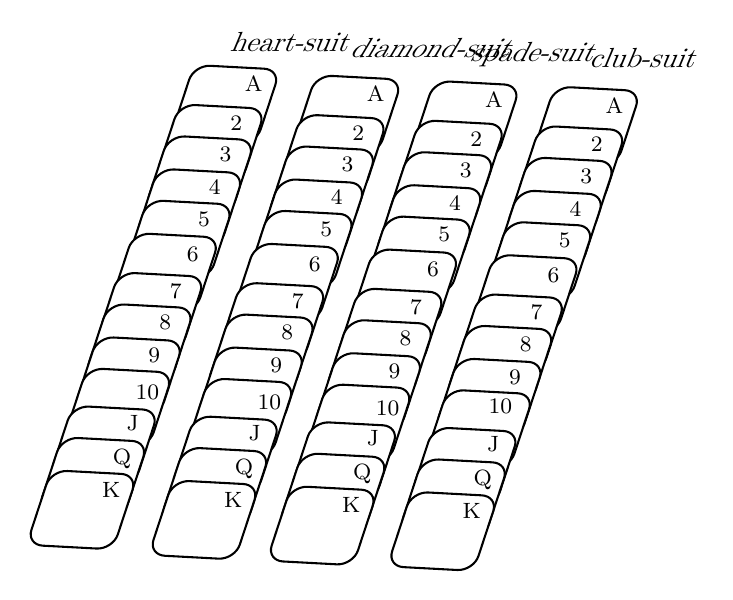
\begin{tikzpicture}[x=0.75pt,y=0.75pt,yscale=-1,xscale=1]
%uncomment if require: \path (0,300); %set diagram left start at 0, and has height of 300

%Rounded Rect [id:dp6128576032908483] 
\draw  [fill={rgb, 255:red, 255; green, 255; blue, 255 }  ,fill opacity=1 ] (243.85,34.05) .. controls (248.17,34.28) and (250.62,37.69) .. (249.31,41.66) -- (242.21,63.24) .. controls (240.91,67.21) and (236.34,70.25) .. (232.01,70.02) -- (206.07,68.64) .. controls (201.75,68.41) and (199.3,65) .. (200.6,61.03) -- (207.7,39.45) .. controls (209.01,35.48) and (213.58,32.44) .. (217.91,32.67) -- cycle ;
%Rounded Rect [id:dp7795928017300927] 
\draw  [fill={rgb, 255:red, 255; green, 255; blue, 255 }  ,fill opacity=1 ] (236.78,52.97) .. controls (241.11,53.2) and (243.56,56.6) .. (242.25,60.58) -- (235.15,82.16) .. controls (233.84,86.13) and (229.27,89.17) .. (224.95,88.94) -- (199.01,87.56) .. controls (194.68,87.33) and (192.23,83.92) .. (193.54,79.95) -- (200.64,58.37) .. controls (201.95,54.39) and (206.51,51.36) .. (210.84,51.59) -- cycle ;
%Rounded Rect [id:dp38096446948076257] 
\draw  [fill={rgb, 255:red, 255; green, 255; blue, 255 }  ,fill opacity=1 ] (231.68,68.1) .. controls (236,68.33) and (238.45,71.74) .. (237.15,75.71) -- (230.05,97.29) .. controls (228.74,101.26) and (224.17,104.3) .. (219.84,104.07) -- (193.9,102.69) .. controls (189.58,102.46) and (187.13,99.05) .. (188.44,95.08) -- (195.54,73.5) .. controls (196.84,69.53) and (201.41,66.49) .. (205.74,66.72) -- cycle ;
%Rounded Rect [id:dp5901650766630238] 
\draw  [fill={rgb, 255:red, 255; green, 255; blue, 255 }  ,fill opacity=1 ] (226.46,83.99) .. controls (230.78,84.22) and (233.23,87.63) .. (231.92,91.6) -- (224.82,113.18) .. controls (223.52,117.15) and (218.95,120.19) .. (214.62,119.96) -- (188.68,118.58) .. controls (184.36,118.35) and (181.91,114.94) .. (183.21,110.97) -- (190.31,89.39) .. controls (191.62,85.42) and (196.19,82.38) .. (200.52,82.61) -- cycle ;
%Rounded Rect [id:dp16189410272363214] 
\draw  [fill={rgb, 255:red, 255; green, 255; blue, 255 }  ,fill opacity=1 ] (221.35,99.12) .. controls (225.68,99.35) and (228.13,102.76) .. (226.82,106.73) -- (219.72,128.31) .. controls (218.41,132.29) and (213.85,135.32) .. (209.52,135.09) -- (183.58,133.71) .. controls (179.25,133.48) and (176.8,130.08) .. (178.11,126.1) -- (185.21,104.52) .. controls (186.52,100.55) and (191.09,97.51) .. (195.41,97.74) -- cycle ;
%Rounded Rect [id:dp42326113968840884] 
\draw  [fill={rgb, 255:red, 255; green, 255; blue, 255 }  ,fill opacity=1 ] (214.76,115.01) .. controls (219.09,115.24) and (221.53,118.65) .. (220.23,122.62) -- (213.13,144.2) .. controls (211.82,148.18) and (207.25,151.21) .. (202.92,150.98) -- (176.99,149.6) .. controls (172.66,149.37) and (170.21,145.97) .. (171.52,141.99) -- (178.62,120.41) .. controls (179.92,116.44) and (184.49,113.4) .. (188.82,113.63) -- cycle ;
%Rounded Rect [id:dp4185585313318074] 
\draw  [fill={rgb, 255:red, 255; green, 255; blue, 255 }  ,fill opacity=1 ] (207.69,133.93) .. controls (212.02,134.16) and (214.47,137.56) .. (213.16,141.54) -- (206.06,163.12) .. controls (204.75,167.09) and (200.19,170.13) .. (195.86,169.9) -- (169.92,168.52) .. controls (165.59,168.29) and (163.14,164.88) .. (164.45,160.91) -- (171.55,139.33) .. controls (172.86,135.35) and (177.43,132.32) .. (181.75,132.55) -- cycle ;
%Rounded Rect [id:dp2920259914907978] 
\draw  [fill={rgb, 255:red, 255; green, 255; blue, 255 }  ,fill opacity=1 ] (202.59,149.06) .. controls (206.92,149.29) and (209.37,152.7) .. (208.06,156.67) -- (200.96,178.25) .. controls (199.65,182.23) and (195.08,185.26) .. (190.76,185.03) -- (164.82,183.65) .. controls (160.49,183.42) and (158.04,180.02) .. (159.35,176.04) -- (166.45,154.46) .. controls (167.76,150.49) and (172.32,147.45) .. (176.65,147.68) -- cycle ;
%Rounded Rect [id:dp7997610326122214] 
\draw  [fill={rgb, 255:red, 255; green, 255; blue, 255 }  ,fill opacity=1 ] (197.37,164.95) .. controls (201.7,165.18) and (204.14,168.59) .. (202.84,172.56) -- (195.74,194.14) .. controls (194.43,198.12) and (189.86,201.15) .. (185.53,200.92) -- (159.6,199.54) .. controls (155.27,199.31) and (152.82,195.91) .. (154.13,191.93) -- (161.23,170.35) .. controls (162.53,166.38) and (167.1,163.34) .. (171.43,163.57) -- cycle ;
%Rounded Rect [id:dp9067963707796727] 
\draw  [fill={rgb, 255:red, 255; green, 255; blue, 255 }  ,fill opacity=1 ] (192.27,180.08) .. controls (196.59,180.31) and (199.04,183.72) .. (197.73,187.69) -- (190.63,209.28) .. controls (189.33,213.25) and (184.76,216.28) .. (180.43,216.05) -- (154.49,214.68) .. controls (150.17,214.45) and (147.72,211.04) .. (149.02,207.07) -- (156.12,185.48) .. controls (157.43,181.51) and (162,178.48) .. (166.33,178.71) -- cycle ;
%Rounded Rect [id:dp21577273271752628] 
\draw  [fill={rgb, 255:red, 255; green, 255; blue, 255 }  ,fill opacity=1 ] (185.32,198.24) .. controls (189.64,198.47) and (192.09,201.88) .. (190.79,205.85) -- (183.69,227.43) .. controls (182.38,231.41) and (177.81,234.44) .. (173.48,234.21) -- (147.55,232.84) .. controls (143.22,232.61) and (140.77,229.2) .. (142.08,225.22) -- (149.18,203.64) .. controls (150.48,199.67) and (155.05,196.64) .. (159.38,196.86) -- cycle ;
%Rounded Rect [id:dp20615672324075307] 
\draw  [fill={rgb, 255:red, 255; green, 255; blue, 255 }  ,fill opacity=1 ] (180.21,213.38) .. controls (184.54,213.61) and (186.99,217.01) .. (185.68,220.99) -- (178.58,242.57) .. controls (177.28,246.54) and (172.71,249.58) .. (168.38,249.35) -- (142.44,247.97) .. controls (138.11,247.74) and (135.67,244.33) .. (136.97,240.36) -- (144.07,218.78) .. controls (145.38,214.8) and (149.95,211.77) .. (154.28,212) -- cycle ;
%Rounded Rect [id:dp3546346081182864] 
\draw  [fill={rgb, 255:red, 255; green, 255; blue, 255 }  ,fill opacity=1 ] (174.99,229.27) .. controls (179.32,229.5) and (181.77,232.9) .. (180.46,236.88) -- (173.36,258.46) .. controls (172.05,262.43) and (167.49,265.47) .. (163.16,265.24) -- (137.22,263.86) .. controls (132.89,263.63) and (130.44,260.22) .. (131.75,256.25) -- (138.85,234.67) .. controls (140.16,230.69) and (144.73,227.66) .. (149.05,227.89) -- cycle ;
%Rounded Rect [id:dp8917377453290999] 
\draw  [fill={rgb, 255:red, 255; green, 255; blue, 255 }  ,fill opacity=1 ] (302.63,38.92) .. controls (306.96,39.15) and (309.41,42.56) .. (308.1,46.53) -- (301,68.12) .. controls (299.69,72.09) and (295.13,75.12) .. (290.8,74.89) -- (264.86,73.52) .. controls (260.53,73.29) and (258.08,69.88) .. (259.39,65.91) -- (266.49,44.32) .. controls (267.8,40.35) and (272.36,37.32) .. (276.69,37.55) -- cycle ;
%Rounded Rect [id:dp2208950823157233] 
\draw  [fill={rgb, 255:red, 255; green, 255; blue, 255 }  ,fill opacity=1 ] (295.57,57.84) .. controls (299.89,58.07) and (302.34,61.48) .. (301.03,65.45) -- (293.93,87.03) .. controls (292.63,91) and (288.06,94.04) .. (283.73,93.81) -- (257.79,92.43) .. controls (253.47,92.2) and (251.02,88.79) .. (252.32,84.82) -- (259.42,63.24) .. controls (260.73,59.27) and (265.3,56.23) .. (269.63,56.46) -- cycle ;
%Rounded Rect [id:dp7590972467883634] 
\draw  [fill={rgb, 255:red, 255; green, 255; blue, 255 }  ,fill opacity=1 ] (290.46,72.97) .. controls (294.79,73.2) and (297.24,76.61) .. (295.93,80.58) -- (288.83,102.16) .. controls (287.52,106.14) and (282.96,109.17) .. (278.63,108.94) -- (252.69,107.57) .. controls (248.36,107.34) and (245.91,103.93) .. (247.22,99.95) -- (254.32,78.37) .. controls (255.63,74.4) and (260.2,71.37) .. (264.52,71.59) -- cycle ;
%Rounded Rect [id:dp2711627981575816] 
\draw  [fill={rgb, 255:red, 255; green, 255; blue, 255 }  ,fill opacity=1 ] (285.24,88.86) .. controls (289.57,89.09) and (292.02,92.5) .. (290.71,96.47) -- (283.61,118.05) .. controls (282.3,122.03) and (277.74,125.06) .. (273.41,124.83) -- (247.47,123.45) .. controls (243.14,123.22) and (240.69,119.82) .. (242,115.84) -- (249.1,94.26) .. controls (250.41,90.29) and (254.98,87.25) .. (259.3,87.48) -- cycle ;
%Rounded Rect [id:dp23825909007295665] 
\draw  [fill={rgb, 255:red, 255; green, 255; blue, 255 }  ,fill opacity=1 ] (280.14,104) .. controls (284.47,104.22) and (286.91,107.63) .. (285.61,111.61) -- (278.51,133.19) .. controls (277.2,137.16) and (272.63,140.2) .. (268.3,139.97) -- (242.37,138.59) .. controls (238.04,138.36) and (235.59,134.95) .. (236.9,130.98) -- (244,109.4) .. controls (245.3,105.42) and (249.87,102.39) .. (254.2,102.62) -- cycle ;
%Rounded Rect [id:dp07362516789869411] 
\draw  [fill={rgb, 255:red, 255; green, 255; blue, 255 }  ,fill opacity=1 ] (273.54,119.88) .. controls (277.87,120.11) and (280.32,123.52) .. (279.01,127.5) -- (271.91,149.08) .. controls (270.61,153.05) and (266.04,156.08) .. (261.71,155.85) -- (235.77,154.48) .. controls (231.44,154.25) and (229,150.84) .. (230.3,146.87) -- (237.4,125.29) .. controls (238.71,121.31) and (243.28,118.28) .. (247.61,118.51) -- cycle ;
%Rounded Rect [id:dp5777585743427922] 
\draw  [fill={rgb, 255:red, 255; green, 255; blue, 255 }  ,fill opacity=1 ] (266.48,138.8) .. controls (270.81,139.03) and (273.25,142.44) .. (271.95,146.41) -- (264.85,167.99) .. controls (263.54,171.97) and (258.97,175) .. (254.65,174.77) -- (228.71,173.39) .. controls (224.38,173.16) and (221.93,169.76) .. (223.24,165.78) -- (230.34,144.2) .. controls (231.64,140.23) and (236.21,137.19) .. (240.54,137.42) -- cycle ;
%Rounded Rect [id:dp32566653068254103] 
\draw  [fill={rgb, 255:red, 255; green, 255; blue, 255 }  ,fill opacity=1 ] (261.38,153.93) .. controls (265.7,154.16) and (268.15,157.57) .. (266.84,161.54) -- (259.74,183.13) .. controls (258.44,187.1) and (253.87,190.13) .. (249.54,189.9) -- (223.6,188.53) .. controls (219.28,188.3) and (216.83,184.89) .. (218.13,180.92) -- (225.23,159.33) .. controls (226.54,155.36) and (231.11,152.33) .. (235.44,152.56) -- cycle ;
%Rounded Rect [id:dp6945029046945058] 
\draw  [fill={rgb, 255:red, 255; green, 255; blue, 255 }  ,fill opacity=1 ] (256.15,169.82) .. controls (260.48,170.05) and (262.93,173.46) .. (261.62,177.43) -- (254.52,199.02) .. controls (253.22,202.99) and (248.65,206.02) .. (244.32,205.79) -- (218.38,204.42) .. controls (214.05,204.19) and (211.61,200.78) .. (212.91,196.81) -- (220.01,175.22) .. controls (221.32,171.25) and (225.89,168.22) .. (230.22,168.45) -- cycle ;
%Rounded Rect [id:dp4709488794155279] 
\draw  [fill={rgb, 255:red, 255; green, 255; blue, 255 }  ,fill opacity=1 ] (251.05,184.96) .. controls (255.38,185.19) and (257.83,188.59) .. (256.52,192.57) -- (249.42,214.15) .. controls (248.11,218.12) and (243.55,221.16) .. (239.22,220.93) -- (213.28,219.55) .. controls (208.95,219.32) and (206.5,215.91) .. (207.81,211.94) -- (214.91,190.36) .. controls (216.22,186.38) and (220.78,183.35) .. (225.11,183.58) -- cycle ;
%Rounded Rect [id:dp16409079980236996] 
\draw  [fill={rgb, 255:red, 255; green, 255; blue, 255 }  ,fill opacity=1 ] (244.1,203.12) .. controls (248.43,203.35) and (250.88,206.75) .. (249.57,210.73) -- (242.47,232.31) .. controls (241.17,236.28) and (236.6,239.32) .. (232.27,239.09) -- (206.33,237.71) .. controls (202,237.48) and (199.55,234.07) .. (200.86,230.1) -- (207.96,208.52) .. controls (209.27,204.54) and (213.84,201.51) .. (218.16,201.74) -- cycle ;
%Rounded Rect [id:dp3388631409567209] 
\draw  [fill={rgb, 255:red, 255; green, 255; blue, 255 }  ,fill opacity=1 ] (239,218.25) .. controls (243.33,218.48) and (245.78,221.89) .. (244.47,225.86) -- (237.37,247.44) .. controls (236.06,251.41) and (231.49,254.45) .. (227.17,254.22) -- (201.23,252.84) .. controls (196.9,252.61) and (194.45,249.21) .. (195.76,245.23) -- (202.86,223.65) .. controls (204.17,219.68) and (208.73,216.64) .. (213.06,216.87) -- cycle ;
%Rounded Rect [id:dp43204958512816616] 
\draw  [fill={rgb, 255:red, 255; green, 255; blue, 255 }  ,fill opacity=1 ] (233.78,234.14) .. controls (238.11,234.37) and (240.56,237.78) .. (239.25,241.75) -- (232.15,263.33) .. controls (230.84,267.3) and (226.27,270.34) .. (221.95,270.11) -- (196.01,268.73) .. controls (191.68,268.5) and (189.23,265.09) .. (190.54,261.12) -- (197.64,239.54) .. controls (198.94,235.57) and (203.51,232.53) .. (207.84,232.76) -- cycle ;
%Rounded Rect [id:dp7661890445479147] 
\draw  [fill={rgb, 255:red, 255; green, 255; blue, 255 }  ,fill opacity=1 ] (359.58,41.66) .. controls (363.91,41.89) and (366.36,45.3) .. (365.05,49.27) -- (357.95,70.85) .. controls (356.65,74.83) and (352.08,77.86) .. (347.75,77.63) -- (321.81,76.25) .. controls (317.49,76.02) and (315.04,72.62) .. (316.34,68.64) -- (323.44,47.06) .. controls (324.75,43.09) and (329.32,40.05) .. (333.65,40.28) -- cycle ;
%Rounded Rect [id:dp41633103341228417] 
\draw  [fill={rgb, 255:red, 255; green, 255; blue, 255 }  ,fill opacity=1 ] (352.52,60.58) .. controls (356.85,60.81) and (359.3,64.21) .. (357.99,68.19) -- (350.89,89.77) .. controls (349.58,93.74) and (345.01,96.78) .. (340.69,96.55) -- (314.75,95.17) .. controls (310.42,94.94) and (307.97,91.53) .. (309.28,87.56) -- (316.38,65.98) .. controls (317.69,62) and (322.25,58.97) .. (326.58,59.2) -- cycle ;
%Rounded Rect [id:dp7210888085066917] 
\draw  [fill={rgb, 255:red, 255; green, 255; blue, 255 }  ,fill opacity=1 ] (347.42,75.71) .. controls (351.74,75.94) and (354.19,79.35) .. (352.89,83.32) -- (345.79,104.9) .. controls (344.48,108.87) and (339.91,111.91) .. (335.58,111.68) -- (309.64,110.3) .. controls (305.32,110.07) and (302.87,106.66) .. (304.17,102.69) -- (311.27,81.11) .. controls (312.58,77.14) and (317.15,74.1) .. (321.48,74.33) -- cycle ;
%Rounded Rect [id:dp9483720676140747] 
\draw  [fill={rgb, 255:red, 255; green, 255; blue, 255 }  ,fill opacity=1 ] (342.2,91.6) .. controls (346.52,91.83) and (348.97,95.24) .. (347.66,99.21) -- (340.56,120.79) .. controls (339.26,124.76) and (334.69,127.8) .. (330.36,127.57) -- (304.42,126.19) .. controls (300.1,125.96) and (297.65,122.55) .. (298.95,118.58) -- (306.05,97) .. controls (307.36,93.03) and (311.93,89.99) .. (316.26,90.22) -- cycle ;
%Rounded Rect [id:dp8664078580240527] 
\draw  [fill={rgb, 255:red, 255; green, 255; blue, 255 }  ,fill opacity=1 ] (337.09,106.73) .. controls (341.42,106.96) and (343.87,110.37) .. (342.56,114.34) -- (335.46,135.92) .. controls (334.15,139.9) and (329.59,142.93) .. (325.26,142.7) -- (299.32,141.32) .. controls (294.99,141.09) and (292.54,137.69) .. (293.85,133.71) -- (300.95,112.13) .. controls (302.26,108.16) and (306.83,105.12) .. (311.15,105.35) -- cycle ;
%Rounded Rect [id:dp43580550170987564] 
\draw  [fill={rgb, 255:red, 255; green, 255; blue, 255 }  ,fill opacity=1 ] (330.5,122.62) .. controls (334.83,122.85) and (337.27,126.26) .. (335.97,130.23) -- (328.87,151.81) .. controls (327.56,155.79) and (322.99,158.82) .. (318.66,158.59) -- (292.73,157.21) .. controls (288.4,156.98) and (285.95,153.58) .. (287.26,149.6) -- (294.36,128.02) .. controls (295.66,124.05) and (300.23,121.01) .. (304.56,121.24) -- cycle ;
%Rounded Rect [id:dp5584197815926703] 
\draw  [fill={rgb, 255:red, 255; green, 255; blue, 255 }  ,fill opacity=1 ] (323.43,141.54) .. controls (327.76,141.77) and (330.21,145.17) .. (328.9,149.15) -- (321.8,170.73) .. controls (320.49,174.7) and (315.93,177.74) .. (311.6,177.51) -- (285.66,176.13) .. controls (281.33,175.9) and (278.88,172.49) .. (280.19,168.52) -- (287.29,146.94) .. controls (288.6,142.96) and (293.17,139.93) .. (297.49,140.16) -- cycle ;
%Rounded Rect [id:dp8661838019763981] 
\draw  [fill={rgb, 255:red, 255; green, 255; blue, 255 }  ,fill opacity=1 ] (318.33,156.67) .. controls (322.66,156.9) and (325.11,160.31) .. (323.8,164.28) -- (316.7,185.86) .. controls (315.39,189.84) and (310.82,192.87) .. (306.5,192.64) -- (280.56,191.26) .. controls (276.23,191.03) and (273.78,187.63) .. (275.09,183.65) -- (282.19,162.07) .. controls (283.49,158.1) and (288.06,155.06) .. (292.39,155.29) -- cycle ;
%Rounded Rect [id:dp9508845146912172] 
\draw  [fill={rgb, 255:red, 255; green, 255; blue, 255 }  ,fill opacity=1 ] (313.11,172.56) .. controls (317.44,172.79) and (319.88,176.2) .. (318.58,180.17) -- (311.48,201.75) .. controls (310.17,205.73) and (305.6,208.76) .. (301.27,208.53) -- (275.34,207.15) .. controls (271.01,206.92) and (268.56,203.52) .. (269.87,199.54) -- (276.97,177.96) .. controls (278.27,173.99) and (282.84,170.95) .. (287.17,171.18) -- cycle ;
%Rounded Rect [id:dp32216690729736597] 
\draw  [fill={rgb, 255:red, 255; green, 255; blue, 255 }  ,fill opacity=1 ] (308,187.69) .. controls (312.33,187.92) and (314.78,191.33) .. (313.47,195.3) -- (306.37,216.89) .. controls (305.07,220.86) and (300.5,223.89) .. (296.17,223.66) -- (270.23,222.29) .. controls (265.9,222.06) and (263.46,218.65) .. (264.76,214.68) -- (271.86,193.09) .. controls (273.17,189.12) and (277.74,186.09) .. (282.07,186.32) -- cycle ;
%Rounded Rect [id:dp08943760761685893] 
\draw  [fill={rgb, 255:red, 255; green, 255; blue, 255 }  ,fill opacity=1 ] (301.06,205.85) .. controls (305.38,206.08) and (307.83,209.49) .. (306.53,213.46) -- (299.43,235.05) .. controls (298.12,239.02) and (293.55,242.05) .. (289.22,241.82) -- (263.28,240.45) .. controls (258.96,240.22) and (256.51,236.81) .. (257.82,232.84) -- (264.92,211.25) .. controls (266.22,207.28) and (270.79,204.25) .. (275.12,204.48) -- cycle ;
%Rounded Rect [id:dp805662074972429] 
\draw  [fill={rgb, 255:red, 255; green, 255; blue, 255 }  ,fill opacity=1 ] (295.95,220.99) .. controls (300.28,221.22) and (302.73,224.62) .. (301.42,228.6) -- (294.32,250.18) .. controls (293.02,254.15) and (288.45,257.19) .. (284.12,256.96) -- (258.18,255.58) .. controls (253.85,255.35) and (251.41,251.94) .. (252.71,247.97) -- (259.81,226.39) .. controls (261.12,222.41) and (265.69,219.38) .. (270.01,219.61) -- cycle ;
%Rounded Rect [id:dp6144131939434834] 
\draw  [fill={rgb, 255:red, 255; green, 255; blue, 255 }  ,fill opacity=1 ] (290.73,236.88) .. controls (295.06,237.11) and (297.51,240.51) .. (296.2,244.49) -- (289.1,266.07) .. controls (287.79,270.04) and (283.23,273.08) .. (278.9,272.85) -- (252.96,271.47) .. controls (248.63,271.24) and (246.18,267.83) .. (247.49,263.86) -- (254.59,242.28) .. controls (255.9,238.3) and (260.47,235.27) .. (264.79,235.5) -- cycle ;
%Rounded Rect [id:dp2586813936455584] 
\draw  [fill={rgb, 255:red, 255; green, 255; blue, 255 }  ,fill opacity=1 ] (417.62,44.4) .. controls (421.95,44.63) and (424.4,48.03) .. (423.09,52.01) -- (415.99,73.59) .. controls (414.68,77.56) and (410.12,80.6) .. (405.79,80.37) -- (379.85,78.99) .. controls (375.52,78.76) and (373.07,75.35) .. (374.38,71.38) -- (381.48,49.8) .. controls (382.79,45.82) and (387.35,42.79) .. (391.68,43.02) -- cycle ;
%Rounded Rect [id:dp39485740837645134] 
\draw  [fill={rgb, 255:red, 255; green, 255; blue, 255 }  ,fill opacity=1 ] (410.56,63.31) .. controls (414.88,63.54) and (417.33,66.95) .. (416.02,70.92) -- (408.92,92.5) .. controls (407.62,96.48) and (403.05,99.51) .. (398.72,99.28) -- (372.78,97.9) .. controls (368.46,97.68) and (366.01,94.27) .. (367.31,90.29) -- (374.41,68.71) .. controls (375.72,64.74) and (380.29,61.71) .. (384.62,61.93) -- cycle ;
%Rounded Rect [id:dp5643654743213579] 
\draw  [fill={rgb, 255:red, 255; green, 255; blue, 255 }  ,fill opacity=1 ] (405.45,78.45) .. controls (409.78,78.68) and (412.23,82.08) .. (410.92,86.06) -- (403.82,107.64) .. controls (402.51,111.61) and (397.95,114.65) .. (393.62,114.42) -- (367.68,113.04) .. controls (363.35,112.81) and (360.9,109.4) .. (362.21,105.43) -- (369.31,83.85) .. controls (370.62,79.87) and (375.19,76.84) .. (379.51,77.07) -- cycle ;
%Rounded Rect [id:dp031209723571941073] 
\draw  [fill={rgb, 255:red, 255; green, 255; blue, 255 }  ,fill opacity=1 ] (400.23,94.34) .. controls (404.56,94.56) and (407.01,97.97) .. (405.7,101.95) -- (398.6,123.53) .. controls (397.29,127.5) and (392.73,130.54) .. (388.4,130.31) -- (362.46,128.93) .. controls (358.13,128.7) and (355.68,125.29) .. (356.99,121.32) -- (364.09,99.74) .. controls (365.4,95.76) and (369.96,92.73) .. (374.29,92.96) -- cycle ;
%Rounded Rect [id:dp732750954296393] 
\draw  [fill={rgb, 255:red, 255; green, 255; blue, 255 }  ,fill opacity=1 ] (395.13,109.47) .. controls (399.46,109.7) and (401.9,113.11) .. (400.6,117.08) -- (393.5,138.66) .. controls (392.19,142.63) and (387.62,145.67) .. (383.29,145.44) -- (357.36,144.06) .. controls (353.03,143.83) and (350.58,140.42) .. (351.89,136.45) -- (358.99,114.87) .. controls (360.29,110.9) and (364.86,107.86) .. (369.19,108.09) -- cycle ;
%Rounded Rect [id:dp08454114971378346] 
\draw  [fill={rgb, 255:red, 255; green, 255; blue, 255 }  ,fill opacity=1 ] (388.53,125.36) .. controls (392.86,125.59) and (395.31,128.99) .. (394,132.97) -- (386.9,154.55) .. controls (385.6,158.52) and (381.03,161.56) .. (376.7,161.33) -- (350.76,159.95) .. controls (346.43,159.72) and (343.99,156.31) .. (345.29,152.34) -- (352.39,130.76) .. controls (353.7,126.79) and (358.27,123.75) .. (362.6,123.98) -- cycle ;
%Rounded Rect [id:dp9403590024297529] 
\draw  [fill={rgb, 255:red, 255; green, 255; blue, 255 }  ,fill opacity=1 ] (381.47,144.27) .. controls (385.8,144.5) and (388.24,147.91) .. (386.94,151.88) -- (379.84,173.47) .. controls (378.53,177.44) and (373.96,180.47) .. (369.64,180.24) -- (343.7,178.87) .. controls (339.37,178.64) and (336.92,175.23) .. (338.23,171.26) -- (345.33,149.67) .. controls (346.63,145.7) and (351.2,142.67) .. (355.53,142.9) -- cycle ;
%Rounded Rect [id:dp770965513589922] 
\draw  [fill={rgb, 255:red, 255; green, 255; blue, 255 }  ,fill opacity=1 ] (376.37,159.41) .. controls (380.69,159.64) and (383.14,163.04) .. (381.83,167.02) -- (374.73,188.6) .. controls (373.43,192.57) and (368.86,195.61) .. (364.53,195.38) -- (338.59,194) .. controls (334.27,193.77) and (331.82,190.36) .. (333.12,186.39) -- (340.22,164.81) .. controls (341.53,160.83) and (346.1,157.8) .. (350.43,158.03) -- cycle ;
%Rounded Rect [id:dp7870087247791839] 
\draw  [fill={rgb, 255:red, 255; green, 255; blue, 255 }  ,fill opacity=1 ] (371.14,175.3) .. controls (375.47,175.53) and (377.92,178.93) .. (376.61,182.91) -- (369.51,204.49) .. controls (368.21,208.46) and (363.64,211.5) .. (359.31,211.27) -- (333.37,209.89) .. controls (329.04,209.66) and (326.6,206.25) .. (327.9,202.28) -- (335,180.7) .. controls (336.31,176.72) and (340.88,173.69) .. (345.21,173.92) -- cycle ;
%Rounded Rect [id:dp6067583391886342] 
\draw  [fill={rgb, 255:red, 255; green, 255; blue, 255 }  ,fill opacity=1 ] (366.04,190.43) .. controls (370.37,190.66) and (372.82,194.07) .. (371.51,198.04) -- (364.41,219.62) .. controls (363.1,223.6) and (358.54,226.63) .. (354.21,226.4) -- (328.27,225.02) .. controls (323.94,224.79) and (321.49,221.39) .. (322.8,217.41) -- (329.9,195.83) .. controls (331.21,191.86) and (335.77,188.82) .. (340.1,189.05) -- cycle ;
%Rounded Rect [id:dp9836114697741176] 
\draw  [fill={rgb, 255:red, 255; green, 255; blue, 255 }  ,fill opacity=1 ] (359.09,208.59) .. controls (363.42,208.82) and (365.87,212.23) .. (364.56,216.2) -- (357.46,237.78) .. controls (356.16,241.75) and (351.59,244.79) .. (347.26,244.56) -- (321.32,243.18) .. controls (316.99,242.95) and (314.54,239.55) .. (315.85,235.57) -- (322.95,213.99) .. controls (324.26,210.02) and (328.83,206.98) .. (333.15,207.21) -- cycle ;
%Rounded Rect [id:dp4871634892255601] 
\draw  [fill={rgb, 255:red, 255; green, 255; blue, 255 }  ,fill opacity=1 ] (353.99,223.72) .. controls (358.32,223.95) and (360.77,227.36) .. (359.46,231.33) -- (352.36,252.91) .. controls (351.05,256.89) and (346.48,259.92) .. (342.16,259.69) -- (316.22,258.32) .. controls (311.89,258.09) and (309.44,254.68) .. (310.75,250.71) -- (317.85,229.12) .. controls (319.16,225.15) and (323.72,222.12) .. (328.05,222.35) -- cycle ;
%Rounded Rect [id:dp5672151170096975] 
\draw  [fill={rgb, 255:red, 255; green, 255; blue, 255 }  ,fill opacity=1 ] (348.77,239.61) .. controls (353.1,239.84) and (355.54,243.25) .. (354.24,247.22) -- (347.14,268.8) .. controls (345.83,272.78) and (341.26,275.81) .. (336.94,275.58) -- (311,274.2) .. controls (306.67,273.98) and (304.22,270.57) .. (305.53,266.59) -- (312.63,245.01) .. controls (313.93,241.04) and (318.5,238) .. (322.83,238.23) -- cycle ;

% Text Node
\draw (233.12,36.44) node [anchor=north west][inner sep=0.75pt]  [font=\footnotesize] [align=left] {A};
% Text Node
\draw (226.05,55.36) node [anchor=north west][inner sep=0.75pt]  [font=\footnotesize] [align=left] {2};
% Text Node
\draw (220.95,70.49) node [anchor=north west][inner sep=0.75pt]  [font=\footnotesize] [align=left] {3};
% Text Node
\draw (215.73,86.38) node [anchor=north west][inner sep=0.75pt]  [font=\footnotesize] [align=left] {4};
% Text Node
\draw (210.62,101.51) node [anchor=north west][inner sep=0.75pt]  [font=\footnotesize] [align=left] {5};
% Text Node
\draw (205.17,118.41) node [anchor=north west][inner sep=0.75pt]  [font=\footnotesize] [align=left] {6};
% Text Node
\draw (196.96,136.32) node [anchor=north west][inner sep=0.75pt]  [font=\footnotesize] [align=left] {7};
% Text Node
\draw (191.86,151.45) node [anchor=north west][inner sep=0.75pt]  [font=\footnotesize] [align=left] {8};
% Text Node
\draw (186.64,167.34) node [anchor=north west][inner sep=0.75pt]  [font=\footnotesize] [align=left] {9};
% Text Node
\draw (180.48,185.03) node [anchor=north west][inner sep=0.75pt]  [font=\footnotesize] [align=left] {10};
% Text Node
\draw (169.48,215.77) node [anchor=north west][inner sep=0.75pt]  [font=\footnotesize] [align=left] {Q};
% Text Node
\draw (164.26,231.66) node [anchor=north west][inner sep=0.75pt]  [font=\footnotesize] [align=left] {K};
% Text Node
\draw (176.08,199.37) node [anchor=north west][inner sep=0.75pt]  [font=\footnotesize] [align=left] {J};
% Text Node
\draw (291.9,41.31) node [anchor=north west][inner sep=0.75pt]  [font=\footnotesize] [align=left] {A};
% Text Node
\draw (284.84,60.23) node [anchor=north west][inner sep=0.75pt]  [font=\footnotesize] [align=left] {2};
% Text Node
\draw (279.73,75.36) node [anchor=north west][inner sep=0.75pt]  [font=\footnotesize] [align=left] {3};
% Text Node
\draw (274.51,91.25) node [anchor=north west][inner sep=0.75pt]  [font=\footnotesize] [align=left] {4};
% Text Node
\draw (269.41,106.39) node [anchor=north west][inner sep=0.75pt]  [font=\footnotesize] [align=left] {5};
% Text Node
\draw (263.95,123.29) node [anchor=north west][inner sep=0.75pt]  [font=\footnotesize] [align=left] {6};
% Text Node
\draw (255.75,141.19) node [anchor=north west][inner sep=0.75pt]  [font=\footnotesize] [align=left] {7};
% Text Node
\draw (250.65,156.33) node [anchor=north west][inner sep=0.75pt]  [font=\footnotesize] [align=left] {8};
% Text Node
\draw (245.42,172.22) node [anchor=north west][inner sep=0.75pt]  [font=\footnotesize] [align=left] {9};
% Text Node
\draw (239.27,189.91) node [anchor=north west][inner sep=0.75pt]  [font=\footnotesize] [align=left] {10};
% Text Node
\draw (228.27,220.64) node [anchor=north west][inner sep=0.75pt]  [font=\footnotesize] [align=left] {Q};
% Text Node
\draw (223.05,236.53) node [anchor=north west][inner sep=0.75pt]  [font=\footnotesize] [align=left] {K};
% Text Node
\draw (234.87,204.25) node [anchor=north west][inner sep=0.75pt]  [font=\footnotesize] [align=left] {J};
% Text Node
\draw (348.85,44.05) node [anchor=north west][inner sep=0.75pt]  [font=\footnotesize] [align=left] {A};
% Text Node
\draw (341.79,62.97) node [anchor=north west][inner sep=0.75pt]  [font=\footnotesize] [align=left] {2};
% Text Node
\draw (336.69,78.1) node [anchor=north west][inner sep=0.75pt]  [font=\footnotesize] [align=left] {3};
% Text Node
\draw (331.47,93.99) node [anchor=north west][inner sep=0.75pt]  [font=\footnotesize] [align=left] {4};
% Text Node
\draw (326.36,109.12) node [anchor=north west][inner sep=0.75pt]  [font=\footnotesize] [align=left] {5};
% Text Node
\draw (320.91,126.02) node [anchor=north west][inner sep=0.75pt]  [font=\footnotesize] [align=left] {6};
% Text Node
\draw (312.7,143.93) node [anchor=north west][inner sep=0.75pt]  [font=\footnotesize] [align=left] {7};
% Text Node
\draw (307.6,159.06) node [anchor=north west][inner sep=0.75pt]  [font=\footnotesize] [align=left] {8};
% Text Node
\draw (302.38,174.95) node [anchor=north west][inner sep=0.75pt]  [font=\footnotesize] [align=left] {9};
% Text Node
\draw (296.22,192.64) node [anchor=north west][inner sep=0.75pt]  [font=\footnotesize] [align=left] {10};
% Text Node
\draw (285.22,223.38) node [anchor=north west][inner sep=0.75pt]  [font=\footnotesize] [align=left] {Q};
% Text Node
\draw (280,239.27) node [anchor=north west][inner sep=0.75pt]  [font=\footnotesize] [align=left] {K};
% Text Node
\draw (291.82,206.98) node [anchor=north west][inner sep=0.75pt]  [font=\footnotesize] [align=left] {J};
% Text Node
\draw (406.89,46.79) node [anchor=north west][inner sep=0.75pt]  [font=\footnotesize] [align=left] {A};
% Text Node
\draw (399.83,65.7) node [anchor=north west][inner sep=0.75pt]  [font=\footnotesize] [align=left] {2};
% Text Node
\draw (394.72,80.84) node [anchor=north west][inner sep=0.75pt]  [font=\footnotesize] [align=left] {3};
% Text Node
\draw (389.5,96.73) node [anchor=north west][inner sep=0.75pt]  [font=\footnotesize] [align=left] {4};
% Text Node
\draw (384.4,111.86) node [anchor=north west][inner sep=0.75pt]  [font=\footnotesize] [align=left] {5};
% Text Node
\draw (378.94,128.76) node [anchor=north west][inner sep=0.75pt]  [font=\footnotesize] [align=left] {6};
% Text Node
\draw (370.74,146.67) node [anchor=north west][inner sep=0.75pt]  [font=\footnotesize] [align=left] {7};
% Text Node
\draw (365.64,161.8) node [anchor=north west][inner sep=0.75pt]  [font=\footnotesize] [align=left] {8};
% Text Node
\draw (360.41,177.69) node [anchor=north west][inner sep=0.75pt]  [font=\footnotesize] [align=left] {9};
% Text Node
\draw (350.48,191.82) node [anchor=north west][inner sep=0.75pt]  [font=\footnotesize] [align=left] {10};
% Text Node
\draw (343.26,226.11) node [anchor=north west][inner sep=0.75pt]  [font=\footnotesize] [align=left] {Q};
% Text Node
\draw (338.04,242) node [anchor=north west][inner sep=0.75pt]  [font=\footnotesize] [align=left] {K};
% Text Node
\draw (349.86,209.72) node [anchor=north west][inner sep=0.75pt]  [font=\footnotesize] [align=left] {J};
% Text Node
\draw (230.41,14.79) node [anchor=north west][inner sep=0.75pt]  [xslant=0.42] [align=left] {\emoji{heart-suit}};
% Text Node
\draw (347.16,19.79) node [anchor=north west][inner sep=0.75pt]  [xslant=0.51] [align=left] {\emoji{spade-suit}};
% Text Node
\draw (289.91,17.79) node [anchor=north west][inner sep=0.75pt]  [xslant=0.6] [align=left] {\emoji{diamond-suit}};
% Text Node
\draw (403.41,22.79) node [anchor=north west][inner sep=0.75pt]  [xslant=0.42] [align=left] {\emoji{club-suit}};


\end{tikzpicture}
  \end{center}
\begin{enumerate}
    \item ¿De cuántas maneras diferentes podemos sacar tres espadas y dos cartas rojas (diamantes y/o corazones)?

  \begin{solution}
    Notamos que tenemos un problema de combinatoria en dos etapas. Primero, obtenemos las maneras que se pueden sacar 3 espadas de 13 cartas de espadas que tenemos:
    $$C(13,3)=286 \text{ maneras.}$$
    Ahora bien, calculamos las maneras que se pueden obtener 2 cartas rojas, de las 26 cartas rojas que tenemos, es decir: 
    $$C(26,2)=325\text{ maneras.}$$
    Ahora aplicamos el principio del producto: 
    $$C(13,3)\cdot C(26,2)= 286\cdot 325 = 92950 \text{ maneras de sacar 3 espadas y 2 cartas rojas.}$$
  \end{solution} 
    \item ¿De cuántas maneras diferentes podemos sacar un flush (cinco cartas del mismo palo, sin necesariamente ser consecutivas)?
      \begin{solution}
      Ya que el orden no importa, es un problema de combinatoria, es decir: 
      $$C(13,5)= 1287 \text{ maneras diferentes de sacar un flush para cada palo.}$$
      Si en caso nos piden la solución para los 4 palos, entonces simplemente sería: 
      $$4\cdot C(13,5)= 4\cdot 1287 = 5148 \text{ maneras diferentes de sacar un flush.}$$
  \end{solution}
\end{enumerate}